\section{Aufbau und Durchführung}
\label{sec:Aufbau und Durchführung}
Zur Aufnahme der Beugungsfiguren der beiden Einfach- und des Doppelspaltes wird ein Aufbau nach Abbildung \ref{fig:Versuchsanordnung} verwendet.
\begin{figure}[H]
    \centering
    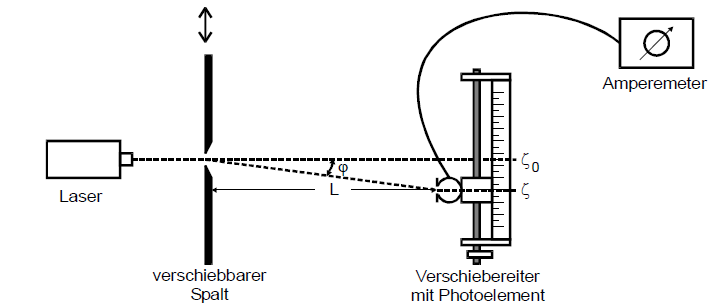
\includegraphics[width=0.8\textwidth]{Versuchsanordnung.png}
    \caption{Versuchsaufbau \cite{1}.}
    \label{fig:Versuchsanordnung}
\end{figure}
\noindent
Als Lichtquelle dient ein Helium-Neon-Laser mit einer Wellenlänge von 633 nm.
 Zur Mesung der Intensitäten wird eine Photodiode verwendet, die einen zur Intensität proportionale Strom erzeugt. 
 Dieser betragsmä"sig sehr geringe Strom wird durch ein Amperemeter gemessen. 
 Zu beachten ist hier noch, dass auch die unbelichtete Photodiode einen gewissen Dunkelstrom abgibt.\\
Die Photodiode kann nun durch eine Mikrometerschraube auf einer Schiene verschoben werden, um die Intensität in Abhängigkeit vom Ort,
 bzw. dem Beugungswinkel anzugeben.

